\chapter{Outcomes and Prospectives}
\label{chap:outcomes}

This internship has yielded valuable insights into optimizing expensive function, and especially the optimization of hyperparameters applied to \acrshort{llm} \gls{fine_tuning}. This chapter start with the presentation and the analysis of the results obtained following the methodology of chapter \ref{chap:methodo}.

Following this presentation, a section will discuss the valorisation of this work in the academic community, i.e. the publication of an article. The scientific contribution along with the redaction of the article will be detailed, as it's crucial in an academic environment to think about the impact of one's work.Looking ahead, this chapter will discuss the challenges faced during experimentation and propose potential areas for future exploration. 



%%%%%%%%%%%%%%%%%%%%%%%%%%%%%%%%%%%%%% Experiments Results %%%%%%%%%%%%%%%%%%%%%%%%%%%%%%%%%%%
\section{Experiment Results}
\label{sec:exp_results}
From what's discussed in chapter \ref{chap:methodo}, three main experiments have been carried out, one by each algorithms (\acrshort{bo}, \acrshort{soo} and \acrshort{bamsoo}). 

To consider and compare experiments results, it's always relevant to define bounds for each metrics, such as unconstrained problem to define lower bound for maximizing combinatorial problem. For this work, I found two bounds : 
\begin{itemize}
    \item Lower bound : experiment with a sampling algorithm (i.e. \acrshort{rs} or \acrshort{lhs}). If complex algorithm does not perform better than sampling ones, it's not worth the complexity. It's especially true in face of expensive objective function, since sampling algorithm are massively parallel.
    \item Upper bound : from Llama-3.2-3B model card\footnote{\href{https://huggingface.co/meta-llama/Llama-3.2-3B}{https://huggingface.co/meta-llama/Llama-3.2-3B}}, \gls{fine_tuning} performance using complex methods (Supervised Fine-Tuning (SFT), Rejection Sampling (RS), and Direct Preference Optimization (DPO)) is available, and can be used as a reference.
\end{itemize}
This approach implied a forth experiment, in section \ref{sec:sampling}, perform a sampling approach with the same budget as other algorithms. As a callback, the evaluation budget of each algorithms is set to 50, including 10 for the sampling part of \acrshort{bo}. The upper and lower bounds values are summarized in table \ref{tab:bounds}, for clarity. This table includes validation and testing dataset, (i.e. Hellaswag and MMLU).


\begin{table}[h]
    \centering
    \begin{tabular}{|c||c|c|}
    \hline
       Datasets  & Lower & Upper \\
    \hline
       Hellaswag  & & 69.8\\
       MMLU & & 63.4\\
    \hline
    \end{tabular}
    \caption{Bounds on accuracy for validation and testing dataset}
    \label{tab:bounds}
\end{table}

%%%%%%%%%%%%%%%%%%%% sampling Experiment %%%%%%%%%%%%%%%%%%%%%%%%%%
\subsection{Sampling experiment}
\label{sec:sampling}



%%%%%%%%%%%%%%%%%%%% BO Experiment %%%%%%%%%%%%%%%%%%%%%%%%%%
\subsection{\acrshort{bo} experiment}
\label{sec:bo_exp}
Figure \ref{fig:exp12_res} depicts the performance of Bayesian Optimization (BO) over 50 iterations, measured in terms of the normalized Hellaswag accuracy (acc\_norm). This visualization highlights the evolution of the optimization process as it transitions from sampling to the exploitation, and ultimately converges towards high-performing solutions.


\begin{figure}[h!]
    \centering
    \begin{subfigure}[b]{.45\textwidth}
      \centering
      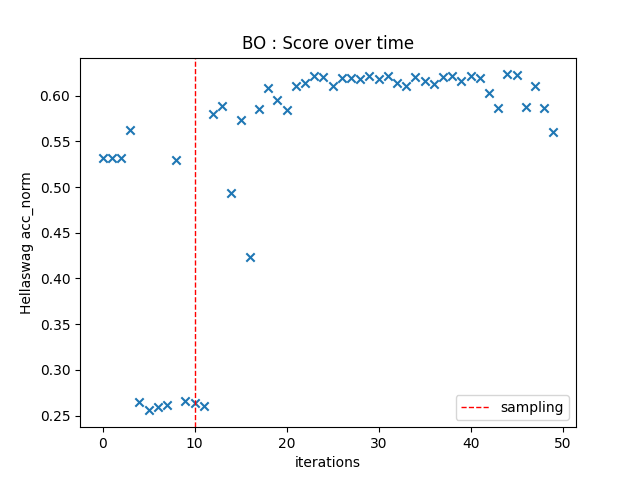
\includegraphics[height = 6cm]{assets/img/chap_4/experiments/plots/exp12_score_over_time.png}
      \caption{Score over time}
      \label{fig:exp12_score_time}
    \end{subfigure}%
    \begin{subfigure}[b]{.45\textwidth}
      \centering
      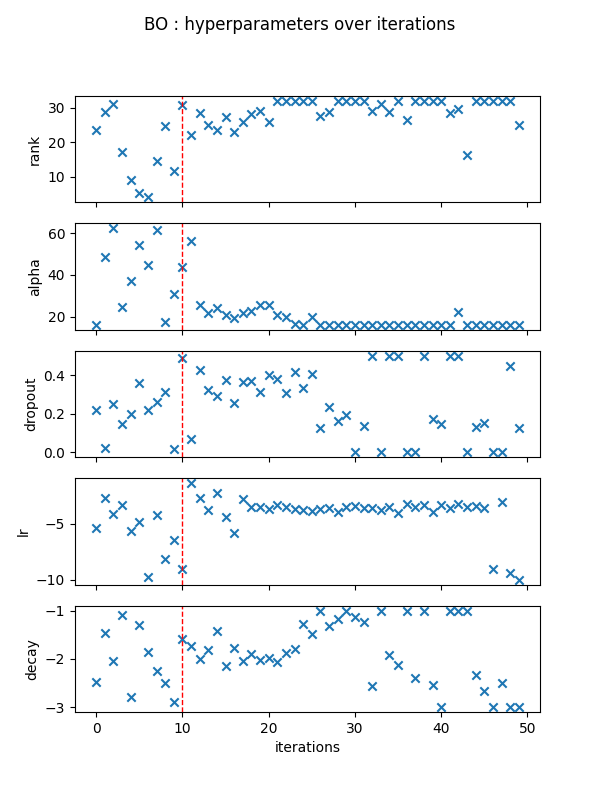
\includegraphics[height = 6cm]{assets/img/chap_4/experiments/plots/exp12_variables_over_time.png}
      \caption{Variable values over time}
      \label{fig:exp12_var_time}
    \end{subfigure}
    \caption{Experiment using \acrshort{bo} algorithm}
    \label{fig:exp12_res}
\end{figure}

During the sampling phase, as shown by figure \ref{fig:exp12_score_time} the best score achieved is at 56.27\% of normalized accuracy. This phase is interesting at is show us that there is a lot of area with good solution without exploitation. After this phase, there is around 15 iterations to converge to a stable phase, around 62\% of accuracy. After 40 iterations, the algorithm renew with a phase of exploration, to look if it's possible to achieve best results in others configuration, resulting in it's decrease in performance.

If we briefly look at figure \ref{fig:exp12_var_time}, it allow to look at well-chosen optimization range, or if it can be useful to enlarge it. For example, when looking at \acrshort{lora} rank, it's keeping it's value at the top of the range, implying that it would go up if possible. 

COMPARE WITH BOUNDS


To summarize, this experiment demonstrate the effectiveness of Bayesian Optimization in efficiently explore the search space. The optimization process strikes a balance between exploration and exploitation, achieving convergence within a limited number of iterations.


%%%%%%%%%%%%%%%%%%%% SOO Experiment %%%%%%%%%%%%%%%%%%%%%%%%%%
\subsection{\acrshort{soo} experiment}
\label{sec:soo_exp}

Figure \ref{fig:soo_score_time} depicts the performance of Simultaneous Optimistic Optimization (SOO) over 50 iterations, measured in terms of the normalized Hellaswag accuracy (acc\_norm). This visualization highlights the progression of the optimization process, showing limited improvement until later iterations, when a significant rise in performance is observed.

\begin{figure}[h!]
    \centering
    \begin{subfigure}[b]{.45\textwidth}
      \centering
      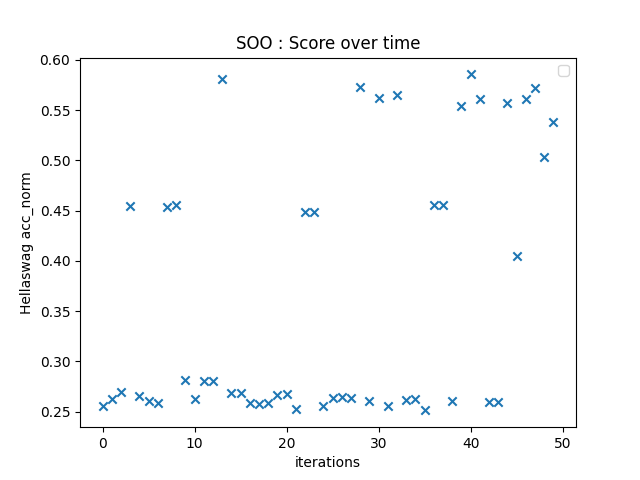
\includegraphics[height = 5cm]{assets/img/chap_4/experiments/plots/exp10_score_over_time.png}
      \caption{Score over time}
      \label{fig:exp11_score_time}
    \end{subfigure}%
    \begin{subfigure}[b]{.45\textwidth}
      \centering
      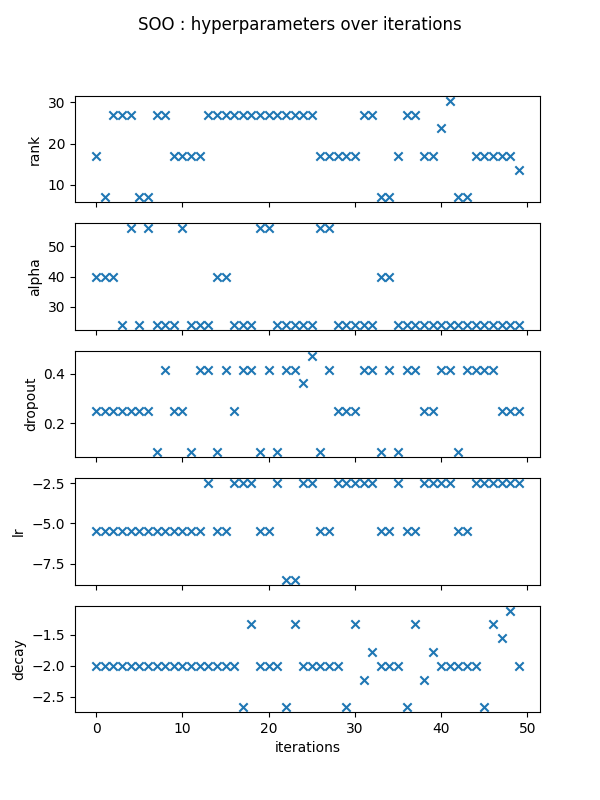
\includegraphics[height = 6cm]{assets/img/chap_4/experiments/plots/exp10_variables_over_time.png}
      \caption{Variables over time}
      \label{fig:exp11_var_time}
    \end{subfigure}
    \caption{Experiment using \acrshort{soo} algorithm}
    \label{fig:exp11_res}
\end{figure}

In the initial phase, spanning roughly the first 20 iterations, the accuracy remains relatively low and consistent, fluctuating around 0.25 to 0.3. This indicates that the SOO algorithm invests heavily in exploration during the early stage, sampling diverse regions of the parameter space but failing to identify high-performing regions.

Between iterations 20 and 40, a gradual improvement is observed as the algorithm transitions to exploitation. In this phase, SOO focuses on refining potential solutions, leading to a slight increase in accuracy, although the improvement remains modest compared to Bayesian Optimization.

In the final stage, after iteration 40, a significant rise in performance is observed, with accuracy values increasing sharply and converging around 0.6. This stabilization phase indicates that SOO successfully identifies high-quality parameter configurations, albeit at a slower pace compared to BO.

To summarize, Figure \ref{fig:soo_score_time} demonstrates that SOO is capable of finding high-performing solutions but requires a longer exploration phase and slower convergence compared to Bayesian Optimization. Despite its delayed success, the eventual convergence highlights the potential of SOO for hyperparameter tuning tasks.

%%%%%%%%%%%%%%%%%%%% BaMSOO Experiment %%%%%%%%%%%%%%%%%%%%%%%%%%
\subsection{\acrshort{bamsoo} experiment}
\label{sec:bamsoo_exp}

Figure \ref{fig:bamsoo_score_time} depicts the performance of Bamsoo over 50 iterations, measured in terms of the normalized Hellaswag accuracy (acc\_norm). This visualization highlights a hybrid approach that balances the rapid improvement seen in Bayesian Optimization (BO) and the thorough exploration typical of Simultaneous Optimistic Optimization (SOO).

\begin{figure}[h!] \centering 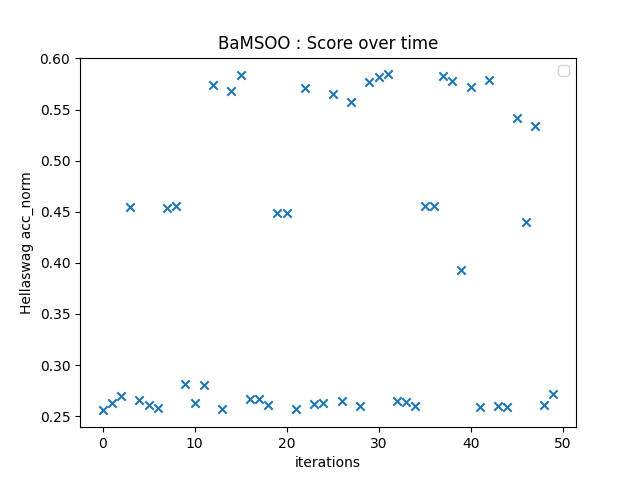
\includegraphics[width=0.4\linewidth]{assets/img/chap_4/experiments/plots/exp11_score_over_time.png} \caption{Score over time with \acrshort{bamsoo}} \label{fig:bamsoo_score_time} \end{figure}

In the initial phase, spanning the first 10 iterations, Bamsoo demonstrates an exploratory behavior similar to SOO. Accuracy values during this phase fluctuate around 0.25 to 0.3, indicating that the algorithm is sampling widely across the parameter space to gather foundational knowledge about the landscape.

Between iterations 10 and 30, the algorithm transitions to a phase of steady improvement, combining elements of exploration and exploitation. This phase is characterized by a gradual rise in accuracy, suggesting that Bamsoo refines its focus on promising regions of the parameter space while still allowing room for broader searches to avoid premature convergence.

In the final stage, after iteration 30, Bamsoo exhibits a stabilization phase with accuracy values consistently converging around 0.55 to 0.6. This indicates that the algorithm successfully identifies high-quality parameter configurations while maintaining the flexibility to avoid getting trapped in local optima.

To summarize, Figure \ref{fig:bamsoo_score_time} illustrates the hybrid nature of Bamsoo, which successfully balances exploration and exploitation across iterations. This behavior enables it to achieve competitive performance relative to BO and SOO, making Bamsoo a compelling alternative for optimization tasks requiring adaptability and robustness.


\section{Article Publication}
\label{sec:article}
The aforementioned results have led to the drafting of a research article aimed at disseminating the findings within the academic community. Publishing the article serves as a means of contributing to the broader field of optimization and machine learning research.

The written article has been submitted to the International Conference on Optimization \& Learning (OLA2025). As of the submission of this report, the paper is under review, and the outcome is awaited.

\section{If This Work Were to Be Continued}
\label{sec:further_work}
While this research represents significant progress, several avenues remain for future exploration:
\begin{itemize}
    \item \textbf{Extending the Search Space:} Expand the range of hyperparameters to include advanced configurations, such as specialized LoRA parameters and task-specific pre-training strategies.
    \item \textbf{Integrating Advanced Techniques:} Investigate the use of cutting-edge approaches, such as reinforcement learning-based optimization or meta-learning, to improve generalization across diverse datasets.
    \item \textbf{Scaling Beyond Current Limits:} Enhance the framework to accommodate even larger LLMs and datasets by leveraging distributed computing infrastructures and more sophisticated partitioning strategies.
\end{itemize}

These directions offer a clear path for further building upon the contributions of this work, ensuring its continued relevance in addressing emerging challenges in the field of LLM fine-tuning and optimization.
